\subtop{Notwendige Datenfelder}{-1.58}
\begin{itemize}
	\item für \decKey~speichern wir für jedes Element eine Boolean-Variable \textit{lost}, zum Speichern, ob bereits ein Kind abgeschnitten wurde
	\item für \exMin~speichern wir für jeden Knoten das Kind mit dem kleinsten Schlüssel
	\item zu jedem Knoten wird das linke und das rechte Kind gespeichert
	\item für \cons~speichern wir die Anzahl der Kinder in der Variablen \textit{degree}
\end{itemize}
\topbreak\ \\\up\up
\begin{minipage}{0.25\textwidth}
	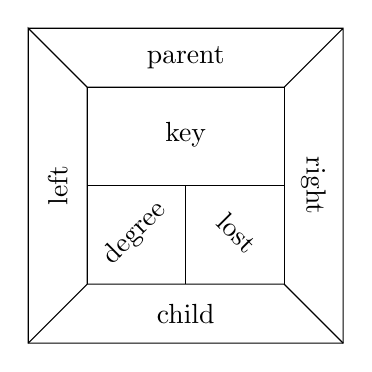
\begin{tikzpicture}[]

\draw[-](0,0)--++(4,0)--++(0,-4)--++(-4,0)--++(0,4)--++(0.75,-0.75)
--++(2.5,0)--++(0.75,0.75);
\draw[-](0.75,-0.75)--++(0,-2.5)--++(-0.75,-0.75);
\draw[-](0.75,0.75-4)--++(2.5,0)--++(0.75,-0.75);
\draw[-](-0.75+4,-4+0.75)--++(0,2.5);
\draw[-](0.75,-2)--++(2.5,0);
\draw[-](0.75+2.5/2,-4+0.75)--++(0,2.5/2);

\node at(2,-0.75/2){parent};
\node at(0.75/2,-2){\rotatebox{90}{left}};
\node at(4-0.75/2,-2){\rotatebox{270}{right}};
\node at(2,-4+0.75/2){\rotatebox{0}{child}};
\node at(2.65,-2.6){\rotatebox{315}{lost}};
\node at(4-2.65,-2.6){\rotatebox{45}{degree}};
\node at(2,-2+0.65){\rotatebox{0}{key}};
\end{tikzpicture}
\end{minipage}
\begin{minipage}{0.7\textwidth}
	Zugehöriger Baum:\\\up\up
	\input{Pics/5_fibheap2.pgf}
\end{minipage}\\\ \\\ \\\ \\